\documentclass[main.tex]{subfiles}

\begin{document}

\section{Aufgabe 1}
Untersuchen Sie, ob folgende Funktionen an der Stelle $x_{0}$ stetig ergänzbar sind:

(a)
\begin{equation*}
    f(x) =\begin{cases}
        2x+1 & \text{für} \ x < -1\\
        4x-1 & \text{für} \ x > -1
    \end{cases} \ \text{und} \ \ x_{0} = -1
\end{equation*}

(b)
\begin{equation*}
    f(x) =x\cdotp \cos\frac{1}{x} \ \ \text{und} \ \ x_{0} = 0
\end{equation*}

(c)
\begin{equation*}
    f(x) =\frac{1}{e^{\frac{1}{x-1}}} \ \ \text{und} \ \ x_{0} = 1
\end{equation*}

\subsection{Lösung 1}
Eine Funktion $f(x)$ ist stetig in einem Punkt $x_{0}$, genau dann wenn
\begin{equation*}
    \lim_{x \uparrow x_{0}} f(x) = \lim_{x \downarrow x_{0}} f(x) = f(x_{0})\text{.}
\end{equation*}

\subsubsection{Lösung 1a}

Zeige Unstetigkeit mit dem Folgenkriterium:\\

Dazu die Folge $r_{n} =-1+\frac{1}{n}$ für die Annäherung von rechts und $l_{n} =-1-\frac{1}{n}$ für die Annäherung von links, da
\begin{equation*}
    \lim_{n\rightarrow \infty } l_{n} =\lim_{n\rightarrow \infty } r_{n} =-1\text{.}
\end{equation*}

Setzt man $r_{n}$ und $l_{n}$ in $f( x)$ für die entsprechenden Bereiche, so erhält man für $x< -1$

\begin{gather*}
    \begin{array}{ c l }
        f( l_{n}) & =2\cdotp l_{n} +1\\
        & =2\cdotp \left( -1-\frac{1}{n}\right) +1\\
        & =-2-\frac{2}{n} +1\\
        & =-\frac{2}{n} -1
    \end{array}\\
    \\
    \lim_{n\rightarrow\infty} f (l_{n}) =\lim_{n\rightarrow\infty} -\frac{2}{n} -1=-1
\end{gather*}
und für $x >-1$
\begin{gather*}
    \begin{array}{ c l }
        f( r_{n}) & =4\cdotp r_{n} -1\\
        & =4\cdotp \left( -1+\frac{1}{n}\right) -1\\
        & =-4+\frac{4}{n} -1\\
        & =-5+\frac{4}{n}
    \end{array}\\
    \\
    \lim_{n\rightarrow\infty} f (r_{n}) =\lim_{n\rightarrow\infty} -5+\frac{4}{n} =-5
\end{gather*}


$\Rightarrow$ Die Funktion $f(x)$ ist an der Stelle $x_{0}$ nicht stetig.

\subsubsection{Lösung 1b}

Die Funktion
\begin{equation*}
    f (x) =x\cdotp \cos\frac{1}{x}
\end{equation*}

ist an der Stelle $x_{0} =0$ nicht definiert $f(x_{0}) \neq 0$, jedoch ist sie stetig ergänzbar, da

\begin{gather*}
    \lim _{x\uparrow x_{0}} f( x) =\lim _{x\uparrow x_{0}}\left( x\cdotp \cos\frac{1}{x}\right) =\underbrace{\lim\limits _{x\uparrow x_{0}} x}_{\rightarrow 0} \cdot \underbrace{\lim\limits _{x\uparrow x_{0}}\cos\frac{1}{x}}_{\rightarrow 0} =0\\
    \\
    \lim _{x\downarrow x_{0}} f( x) =\lim _{x\downarrow x_{0}}\left( x\cdotp \cos\frac{1}{x}\right) =\underbrace{\lim\limits _{x\downarrow x_{0}} x}_{\rightarrow 0} \cdot \underbrace{\lim\limits _{x\downarrow x_{0}}\cos\frac{1}{x}}_{\rightarrow 0} =0
\end{gather*}

gilt und die Funktion daher um $f(x_0) = 0$ ergänzt werden und wie folgt angegeben werden kann:

\begin{equation*}
    f(x) = \begin{cases}
    x\cdot \cos\frac{1}{x} & \text{für} \ x\neq 0\\
    0 & \text{für} \ x=0
    \end{cases}
\end{equation*}

\subsubsection{Lösung 1c}
\begin{figure}[ht]
	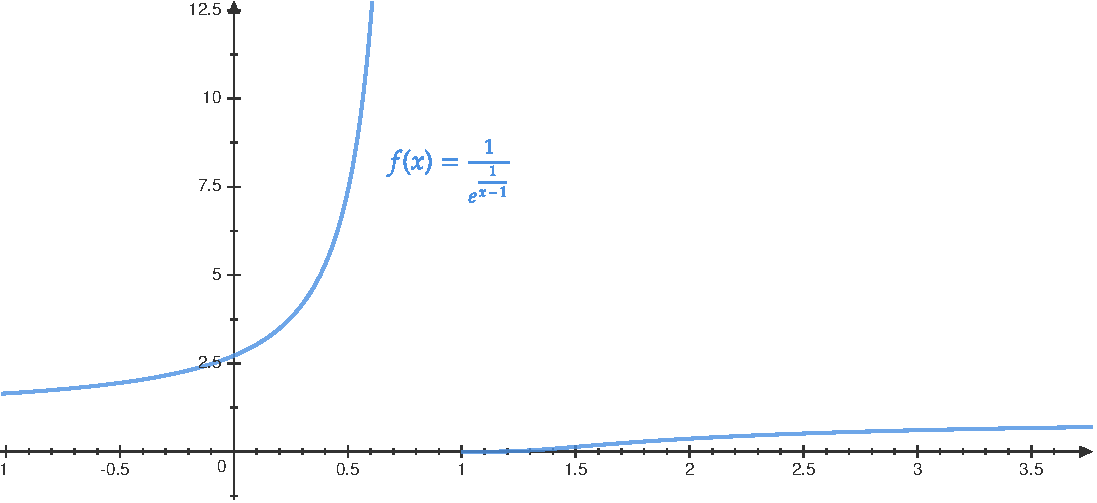
\includegraphics[width=\linewidth]{fig-1c.pdf}
	\caption{Graph von $f(x)$}
\end{figure}

Die Funktion
\begin{equation*}
    f( x) =\frac{1}{e^{\frac{1}{x-1}}}
\end{equation*}
ist an der Stelle $x_{0} =1$ nicht stetig und kann auch nicht stetig ergänzt werden, da
\begin{gather*}
    \lim _{x\uparrow x_{0}} f( x) =\lim _{x\uparrow x_{0}}\left(\frac{1}{e^{\frac{1}{x-1}}}\right) =\underbrace{\lim\limits _{x\uparrow x_{0}}\frac{1}{\underbrace{e^{\underbrace{\frac{1}{x-1}}_{\rightarrow -\infty }}}_{\rightarrow 0}}}_{\rightarrow \infty } =\infty \\
    \\
    \lim _{x\downarrow x_{0}} f( x) =\lim _{x\downarrow x_{0}}\left(\frac{1}{e^{\frac{1}{x-1}}}\right) =\underbrace{\lim\limits _{x\downarrow x_{0}}\frac{1}{\underbrace{e^{\underbrace{\frac{1}{x-1}}_{\rightarrow \infty }}}_{\rightarrow \infty }}}_{\rightarrow 0} =0
\end{gather*}
gilt und somit
\begin{equation*}
    \lim _{x\uparrow x_{0}} f( x) \neq \lim _{x\downarrow x_{0}} f( x)\text{.}
\end{equation*}


\end{document}
